\part{Algebraic Topology}
\section{Math Stackexchange Digest}
\paragraph{1}\href{https://math.stackexchange.com/questions/42005}{Precise official definition of a cell complex and CW-complex}

The defintion of cell complex from Introduction to Topological Manifolds (John M. Lee):

   Here are technical details of the definition. If $X$ is a non-empty topological space, a {\it cell decomposition of} $X$ is a partition $\mathcal{E}$ of $X$ into subspaces that are open cells of various dimensions, such that the following condition is satisfied:
   
   for each cell $e\in \mathcal{E}$ of dimension $n\geq 1$, there exists a continuous map $\phi$
   from some closed $n$-cell $\DD$ into $X$ (called a {\it characteristic map for $e$}) that restricts to a homeomorphism from $D^{\circ}$ (interior) onto $e$ and maps $\partial D$ into the union of all cells of $\mathcal{E}$ of dimensions strictly less than $n$.\par
   A {\it cell complex} is a Hausdorff\footnote{The Hausdorff condition is included both to rule out various pathologies (病理学) and because, as we show below, the inductive construction of cell complexes automatically yields Hausdorff spaces.} space $X$ together with a specific cell decomposition of $X$.\par
   A {\it CW complex} is cell complex $(X,\mathcal{B})$ satisfying the following additional conditions:\\
   (C) The closure of each cell is contained in a union of finitely many cells.\\
   (W) The topology of $X$ is coherent\footnote{First we need the following definition. Suppose $X$ is a topological space, and $\mathcal{B}$ is any family of subspaces of $X$ whose union is $X$. To say that the topology of $X$ is {\it coherent} with $\mathcal{B}$ means that a subset $U\subseteq X$ is open in $X$ if and only if its intersection with each $B\in \mathcal{B}$ is open in $B$.\par 
   It is easy to show by taking complements that this is equivalent to the requirement that $U$ is closed in $X$ if and only if $U\cap B$ is closed in $B$ for each $B \in\mathcal{B}$. (In either case, the "only if" implication always hold by definition of the subspace topology on $B$, so it is the "if" part that is significant. For example, if $(X_{\alpha})$ is an indexed family of topological spaces, the disjoint union topology on $\coprod X_{\alpha}$ is coherent with the family $(X_{\alpha})$, thought of as subspaces of the disjoint union.} with the family of closed subspaces $\{\bar{e}:\ e\in \mathcal{B}\}$ \par
\vspace{3pt}
\hrule
\vspace{3pt}
Let $\mathbb{B}^n$ denote a closed n-ball. As far as I know, a {\it cell complex} is a space, obtained as \[X=\bigcup_{i\in\mathbb{N}_0} X^{(i)},\] 
such that
1. $X^{(0)}$ is a discrete space and

2. $X^{(n)}$ is obtained from $X^{(n-1)}$ by attaching $n$-cells, i.e.
\[X^{(n)}= X^{(n-1)}\bigcup_{f_{\lambda}}\mathbb{B}^n= X^{(n-1)}\coprod \mathbb{B}^n/\sim\]
where $x\sim f_\lambda(x)$.

3. $A\subseteq X$ is closed in $X$ if and only if $A\cap X^{(n)}$ is closed in $X^{(n)}$ for any $n$.

But shouldn't there be some condition on $f_\lambda$? For example, if we have a graph ($1$-dimensional complex) consisting of a single vertex and a single edge. Then when we are attaching $\mathbb{B}^2$, we can set $f$ to map the whole $S^1$ to a single point on the edge, that isn't the vertex. Thus we get a very weird space:
\begin{figure}[h!]
\centering
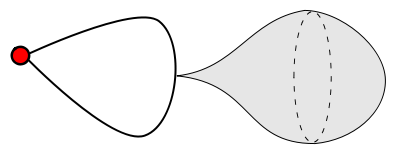
\includegraphics[width=6cm]{hulu.png}
\end{figure}

Shouldn't $f$ go along each loop/edge in $X^{(1)}$ integer many times and not stop in the middle? Also, how do we prevent $f$ from oscillating infninitely? For example, if $X^{(1)}$ contains two edges $a,b\subseteq\{0\}\times\mathbb{R}\subseteq\mathbb{R}^2$ with $a\cap b=\{(0,0)\}$, then $f(x)=(0,x^2\sin(1/x))$ can go infinitely many times into $a$ and $b$.\hfill || \par



No part of the definition of a CW complex prevents the sorts of examples that you have indicated.  In particular:

1. It is perfectly fine for the entire boundary of a 2-cell to be attached to a single point in the middle of a 1-cell.

2. It is perfectly fine for the boundary of a 2-cell to be attached to a 1-cell in an oscillating fashion, e.g. locally resembling $x \sin(1/x)$.\par

I think you have a good understanding of the definition of a CW complex, you are just confused about how a definition this general could be useful.\par

The reason is that algebraic topology is mostly defined up to homotopy equivalence. This is usually defined as follows: two spaces $X$ and $Y$ are homotopy equivalent if there exist maps $f\colon X\to Y$ and $g\colon Y \to X$ so that $f\circ g$ and $g\circ f$ are homotopic to the identity map.  Homotopy equivalent spaces have the same homotopy groups, the same homology and cohomology groups, and essentially all the same homotopical properties.\par

The reason that wildness of the attaching maps $f_\lambda$ is unimportant is that any "wild" CW complex is homotopy equivalent to a "tame" CW complex.  In particular, the homotopy type of a CW complex is entirely determined by the homotopy classes of the attaching maps. That is, if you replace one of the attaching maps by a homotopic map, then the resulting CW complex is homotopy equivalent.\par

For example, if the entire boundary of a 2-cell is attached to the middle of a 1-cell, this is homotopic to a map that attaches the entire boundary to a nearby 0-cell, so the two resulting complexes are homotopy equivalent.  Similarly, any oscillating map like $x\sin(1/x)$ is homotopic to a more reasonable map, so any CW complex with an oscillating attachment is homotopy equivalent to one with nicer attaching maps.\par

Indeed, assuming we are willing to work up to homotopy equivalence, we can assume that the boundary of any 2-cell maps to either

1. A single 0-cell via a constant map, or

2. To a closed loop of edges in the 1-skeleton, using a map which is locally an embedding.\par

This is how topologists tend to think of cell complexes for the purposes of algebraic topology.\par

Incidentally, the reason that it is useful to allow arbitrary attaching maps is that it glosses over (掩盖,避免考虑) the problem of how to choose a "nice" representative for each homotopy class of maps from the boundary of an $n$-cell to the $(n-1)$-skeleton.  Though it's obvious how such "nice" representatives should work when $n=2$, it becomes less clear in higher dimensions.\par

For example, it is possible to have a CW complex whose $2$-skeleton is a 2-sphere, and then attach a $4$-cell to the $2$-skeleton using a non-trivial element of $\pi_3(S^2)$.  That is, the boundary of the $4$-cell is a $3$-sphere $S^3$, which is being attached to the sphere $S^2$ via the [Hopf map][2] $S^3 \to S^2$.  This is actually a very useful cell complex, because it gives a cell structure for the projective space $\mathbb{C}P^2$ with only three cells.\par

Simplicial complexes are much simpler: they are truly just combinatorial objects, with simplexes glued together using the simple linear identifications.  The disadvantage is that a simplicial complex must usually have many more simplices than the cells of a cell complex.  For example, there exists a CW complex for the torus that has only four cells, while a simplical complex homeomorphic to a torus requires at least a couple dozen simplices.  In general, putting a CW structure on a space requires only homotopy information, while putting a simplicial structure on the space requires a much more careful consideration of the geometry.\par

By the way, the best place to learn about cell complexes and their relation to homotopy equivalence is Chapter 0 of \cite{hatcher}.